\documentclass[12pt, oneside]{article}
\usepackage[letterpaper, margin=1in]{geometry}
\usepackage[english]{babel}
\usepackage[utf8]{inputenc}
\usepackage{amsmath}
\usepackage{amsfonts}
\usepackage{amssymb}
\usepackage{tikz}
\usepackage{tkz-fct}

\usepackage{fancyhdr}
\pagestyle{fancy}
\fancyhf{}
\rhead{\thepage \\Name: \hspace{1.5in}.\\}
\lhead{BECA / Dr. Huson / 11.2 Algebra 2 \\* 1 June 2018 \\* \textbf{Final Exam}}

\vspace{1cm}

\renewcommand{\headrulewidth}{0pt}

\title{Problem set template}
\author{Chris Huson}
\date{May 2018}

\begin{document}
%\maketitle

\subsubsection*{\\* \textnormal{This first page must be done from memory. No notes. Answer in pen.}}

\begin{enumerate}

\item Given a loan or investment there are certain values to substitute into one of three formulas. Assume\\[5pt]
\quad Principal amount invested, $P_0= \$1,000$\\[5pt]
\quad Interest rate, $r=5\% = 0.05$\\[5pt]
\quad Time, $t=5$ years \\[5pt]
\quad Compounding periods per year, $n=12$\\[15pt]
For each interest rate convention below, first write the formula, then substitute the values, finally, write down the final balance (use your calculator). 

\begin{enumerate}
    \item Continuous interest \\[1.25in]
    \item Monthly compounded interest \\[1.5in]
\end{enumerate}

\item Explain how $\displaystyle \left(2^{\frac{1}{5}} \right)^3$ can be written as the equivalent radical expression $\sqrt[5]8$. %Alg2 Regents Aug2016


\newpage
\item For each polynomial graph, state 
\begin{enumerate}
\item its degree,
\item how many distinct zeros it has, and
\item the sign of its leading coefficient.
\end{enumerate}

    \begin{tikzpicture}[scale=2/4]
    %\draw[step=1cm,gray,very thin] (-7,-7) grid (7,7);
    \draw[thick,<->] (-7.5,0) -- (7.5,0) node[anchor=north west] {\textbf{x}};
    \draw[thick,<->] (0,-7.5) -- (0,7.5) node[anchor=south east] {\textbf{y}};
    %\foreach \x in {-6, -4, -2, 2, 4, 6} \draw (\x cm,1pt) -- (\x cm,-1pt) node[anchor=north] {$\x$};
    %\foreach \y in {5} \draw (1pt,\y cm) -- (-1pt,\y cm) node[anchor=east] {50}; %{$\y$};
    \tkzInit[xmin=-6,xmax=6,ymin=-7,ymax=7,ystep=1]   
    \tkzFct[color=black,thick,<->,domain = -3.3:5.2] {0.05*(x*x*x*x-3*x*x*x-9*x*x+10*x+20)};
    \end{tikzpicture}
    \begin{tikzpicture}[scale=2/4]
    %\draw[step=1cm,gray,very thin] (-7,-7) grid (7,7);
    \draw[thick,<->] (-7.5,0) -- (7.5,0) node[anchor=north west] {\textbf{x}};
    \draw[thick,<->] (0,-7.5) -- (0,7.5) node[anchor=south east] {\textbf{y}};
    %\foreach \x in {-6, -4, -2, 2, 4, 6} \draw (\x cm,1pt) -- (\x cm,-1pt) node[anchor=north] {$\x$};
    %\foreach \y in {5} \draw (1pt,\y cm) -- (-1pt,\y cm) node[anchor=east] {50}; %{$\y$};
    \tkzInit[xmin=-6,xmax=6,ymin=-7,ymax=7,ystep=1]   
    \tkzFct[color=black,thick,<->,domain = -4.3:5.2] {-0.1*(x+3)*(x)*(x-4)};
    \end{tikzpicture}
\\[30pt]
    \begin{tikzpicture}[scale=2/4]
    %\draw[step=1cm,gray,very thin] (-7,-7) grid (7,7);
    \draw[thick,<->] (-7.5,0) -- (7.5,0) node[anchor=north west] {\textbf{x}};
    \draw[thick,<->] (0,-7.5) -- (0,7.5) node[anchor=south east] {\textbf{y}};
    %\foreach \x in {-6, -4, -2, 2, 4, 6} \draw (\x cm,1pt) -- (\x cm,-1pt) node[anchor=north] {$\x$};
    %\foreach \y in {5} \draw (1pt,\y cm) -- (-1pt,\y cm) node[anchor=east] {50}; %{$\y$};
    \tkzInit[xmin=-6,xmax=6,ymin=-7,ymax=7,ystep=1]   
    \tkzFct[color=black,thick,<->,domain = -5.3:4.2] {-0.05*(x+5)*(x+3)*(x-1)*(x-4)};
    \end{tikzpicture}
    \begin{tikzpicture}[scale=2/4]
    %\draw[step=1cm,gray,very thin] (-7,-7) grid (7,7);
    \draw[thick,<->] (-7.5,0) -- (7.5,0) node[anchor=north west] {\textbf{x}};
    \draw[thick,<->] (0,-7.5) -- (0,7.5) node[anchor=south east] {\textbf{y}};
    %\foreach \x in {-6, -4, -2, 2, 4, 6} \draw (\x cm,1pt) -- (\x cm,-1pt) node[anchor=north] {$\x$};
    %\foreach \y in {5} \draw (1pt,\y cm) -- (-1pt,\y cm) node[anchor=east] {50}; %{$\y$};
    \tkzInit[xmin=-6,xmax=6,ymin=-7,ymax=7,ystep=1]   
    \tkzFct[color=black,thick,<->,domain = -1.3:5.2] {-0.5*(x-2)*(x-2)};
    \end{tikzpicture}


\newpage

\subsubsection*{\textnormal{This section open note. Answer in pen. Show work. Graph carefully using pencil.}}


\item Write $\sqrt[4]x \cdot \sqrt{x}$ as a single term with a rational exponent. %Alg2 Regents Jun2017
\\*[1.75in]


\item Given $i$ is the imaginary unit, $(3-zi)^2$ in simplest form is what? \\[2.5in]%Alg2 Regents Jun2016

\item What is the expression $2ai^3(xi-3)$ is equivalent to?  %Alg2 Regents Jun2017 multiple choice


\newpage
\item Sketch a graph of a cubic polynomial with the following characteristics:
\begin{itemize}
\item three positive, real zeros
\item as $x \rightarrow + \infty$, $f(x) \rightarrow + \infty$
\item as $x \rightarrow - \infty$, $f(x) \rightarrow - \infty$
\end{itemize}
\begin{center}
    \begin{tikzpicture}[scale=2/4]
    \draw[thick,<->] (-7.5,0) -- (7.5,0) node[anchor=north west] {\textbf{x}};
    \draw[thick,<->] (0,-7.5) -- (0,7.5) node[anchor=south east] {\textbf{y}};
    \end{tikzpicture}
\end{center} %Alg2 Regents Jun2016 MC

\item Given: $f(x)=3x^2- x + 2$ and $g(x)=3x+7$\\*[5pt]
Express $2 \bullet g(x) - f(x)$ as a polynomial in standard form. \\[3in] %Alg2 Regents Jan2018

\newpage
\item Find algebraically the zeros for  $g(x)=x^3+x^2-4x-4$.\\*[2in]
On the set of axes below, graph $y=g(x)$.
\begin{center}
    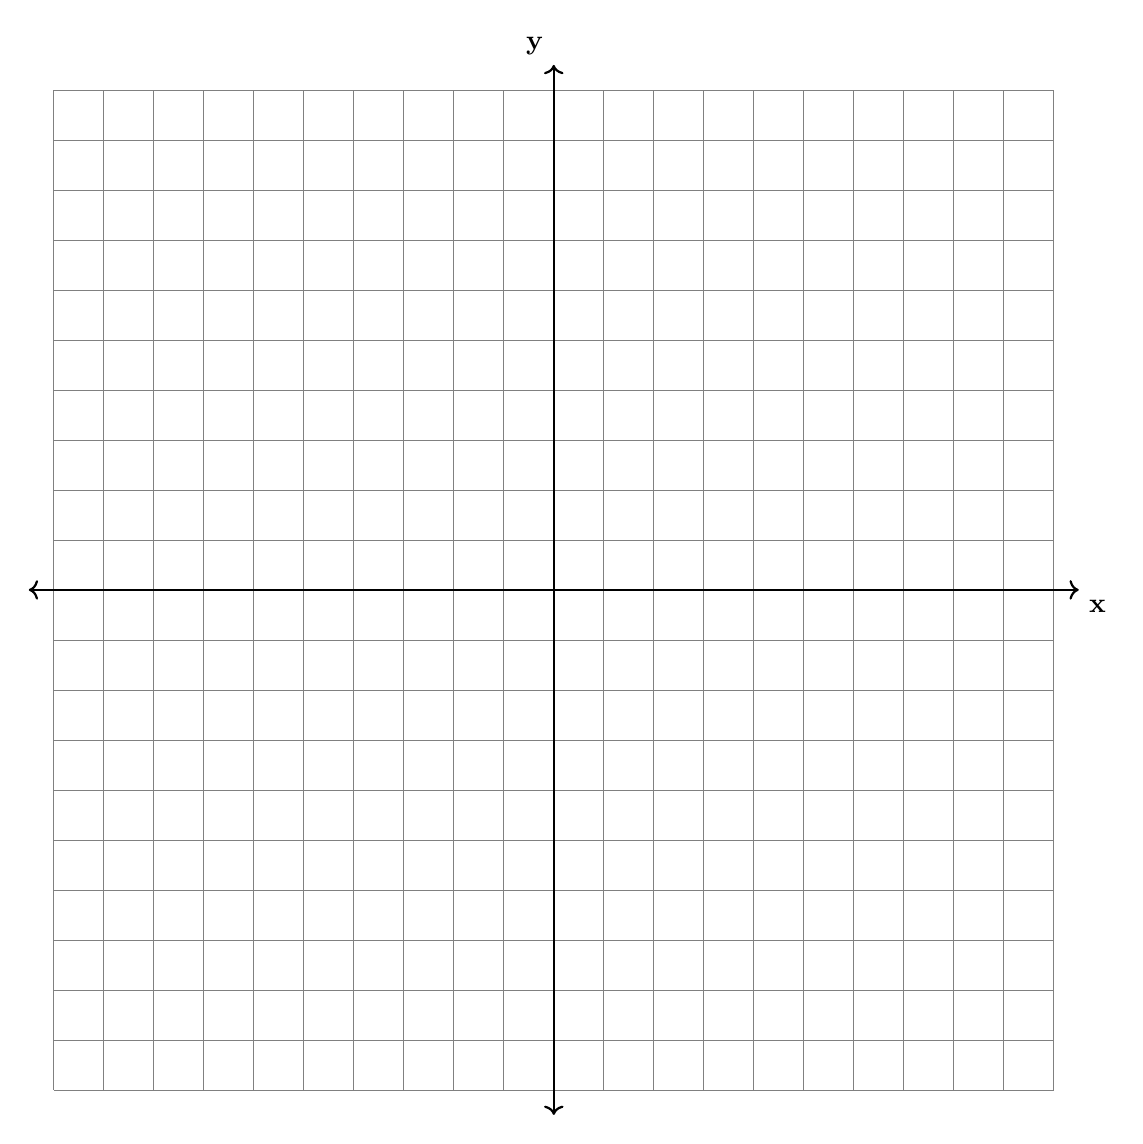
\begin{tikzpicture}[scale=2.54/4]
    \draw[step=1cm,gray,very thin] (-10,-10) grid (10,10);
    \draw[thick,<->] (-10.5,0) -- (10.5,0) node[anchor=north west] {\textbf{x}};
    \draw[thick,<->] (0,-10.5) -- (0,10.5) node[anchor=south east] {\textbf{y}};
    %\foreach \x in {-6, -4, -2, 2, 4, 6} \draw (\x cm,1pt) -- (\x cm,-1pt) node[anchor=north] {$\x$};
    %\foreach \y in {5} \draw (1pt,\y cm) -- (-1pt,\y cm) node[anchor=east] {50};
    %\foreach \y in {-5} \draw (1pt,\y cm) -- (-1pt,\y cm) node[anchor=east] {-50};    \tkzInit[xmin=-5,xmax=5,ymin=-7,ymax=7,ystep=1]
%    \tkzFct[color=black,thick,<->,domain = -3.4:7] {0.1*(x*x-4)*(x-5)};
    \end{tikzpicture}
\end{center} %Alg2 Regents Aug2016



\newpage
\item Using long division, find the quotient and remainder of $\displaystyle \frac{f(x)}{g(x)}$, where $f(x)=3x^2+7x-20$ and $g(x)=x+3$. \\[3in] %Alg2 Regents Jan2017


\item Researchers in a local area found that the population of rabbits with an initial population of 25 grew continuously at the rate of 4\% per month. The fox population had an initial value of 35 and grew continuously at the rate of 2\% per month.\\*[5pt]
Find, to the \emph{nearest tenth of a month}, how long it takes for these populations to be equal. \\[3in] %Alg2 Regents Jan2018

\newpage

\item Jim is looking to buy a vacation home for \$165,000 near his favorite southern beach. The formula to compute a mortgage payment, $M$, is $\displaystyle M=P \cdot \frac{r(1+r)^N}{(1+r)^N-1}$ where $P$ is the principal amount of the loan, $r$ is the monthly interest rate, and $N$ is the number of monthly payments. Jim’s bank offers a monthly interest rate of 0.5\% for a 15-year mortgage.\\*[5pt]
With no down payment, determine Jim’s mortgage payment, rounded to the nearest dollar.\\*[3in]
Algebraically determine and state the down payment, rounded to the \emph{nearest dollar}, that Jim needs to make in order for his mortgage payment to be \$1250.
 %Alg2 Regents Jun2017 multiple choice


\newpage

\item Graph $y=85(1.15)^{0.75x}+25$ on the set of axes below.
\begin{center}
    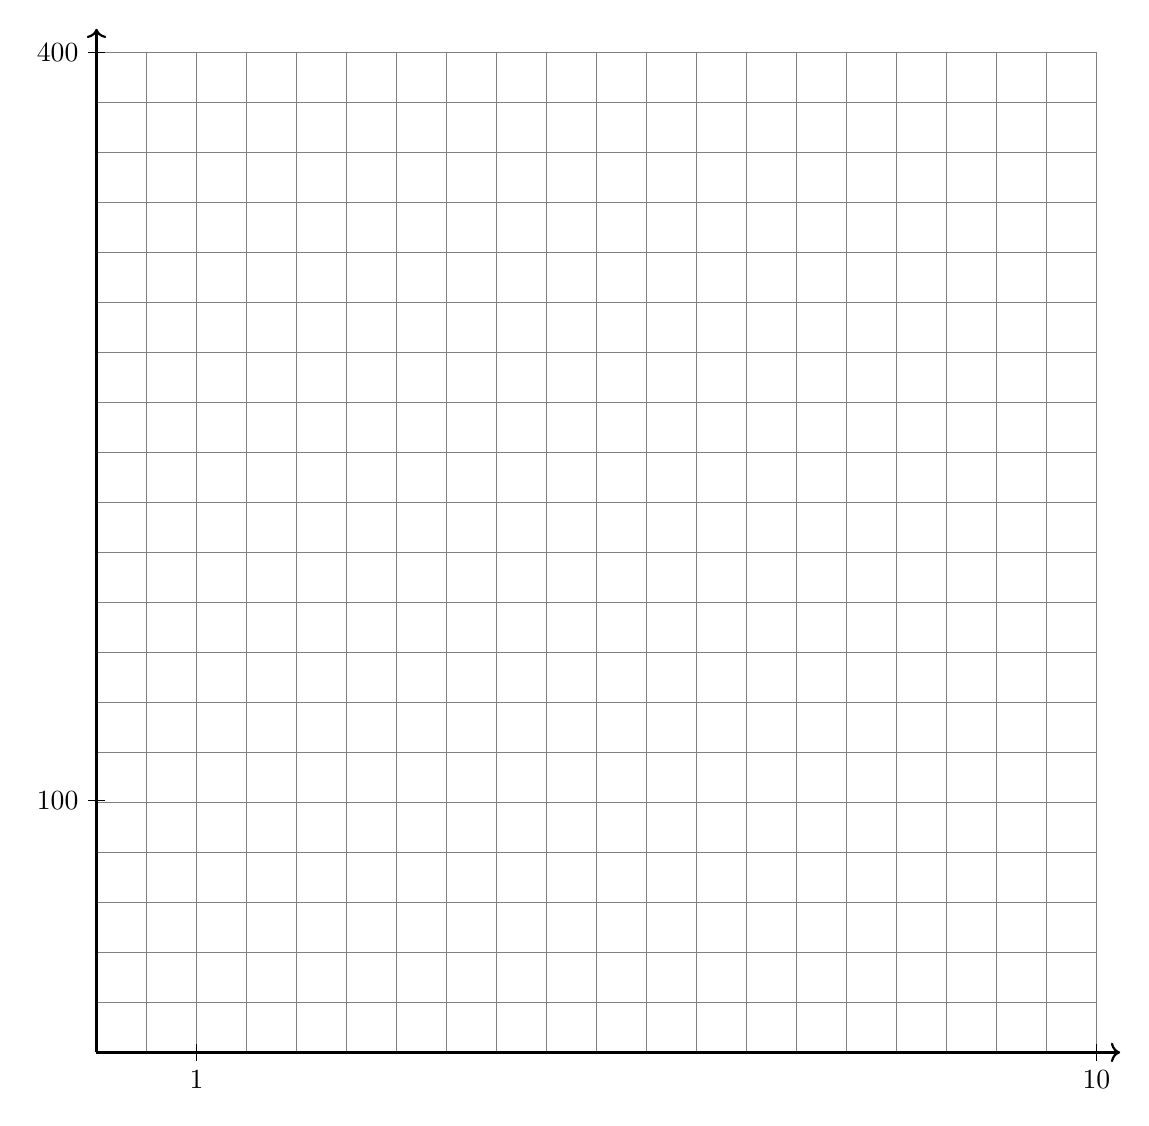
\begin{tikzpicture}
    \draw[step=0.25in,gray,very thin] (0,0) grid (12.7,12.7);
    \draw[thick,->] (0,0) -- (13,0); node[anchor=north west] {x};
    \draw[thick,->] (0,0) -- (0,13); node[anchor=south east] {y};
    \foreach \x in {1.27} \draw (\x cm,3pt) -- (\x cm,-3pt) node[anchor=north] {$1$};
    \foreach \x in {12.7} \draw (\x cm,3pt) -- (\x cm,-3pt) node[anchor=north] {10};
    \foreach \y in {3.2} \draw (3pt,\y cm) -- (-3pt,\y cm) node[anchor=east] {100};
    \foreach \y in {12.7} \draw (3pt,\y cm) -- (-3pt,\y cm) node[anchor=east] {400};
    \end{tikzpicture}
\end{center} %Alg2 Regents Jun2017

\newpage

\newpage
\item The zeros for $f(x)=x^4+4x^3-9x^2-36x$ are
\begin{enumerate}
    \item $\{0, \pm 3, 4 \}$
    \item $\{0, 3, 4 \}$
    \item $\{0, \pm 3, -4 \}$
    \item $\{0, 3,4 \}$
\end{enumerate} %Alg2 Regents Jun2016

\item Which graph has the following characteristics?
\begin{itemize}
\item three real zeros
\item as $x \rightarrow - \infty$, $f(x) \rightarrow - \infty$
\item as $x \rightarrow \infty$, $f(x) \rightarrow - \infty$
\end{itemize}
\begin{figure}[!ht]
    \centering
    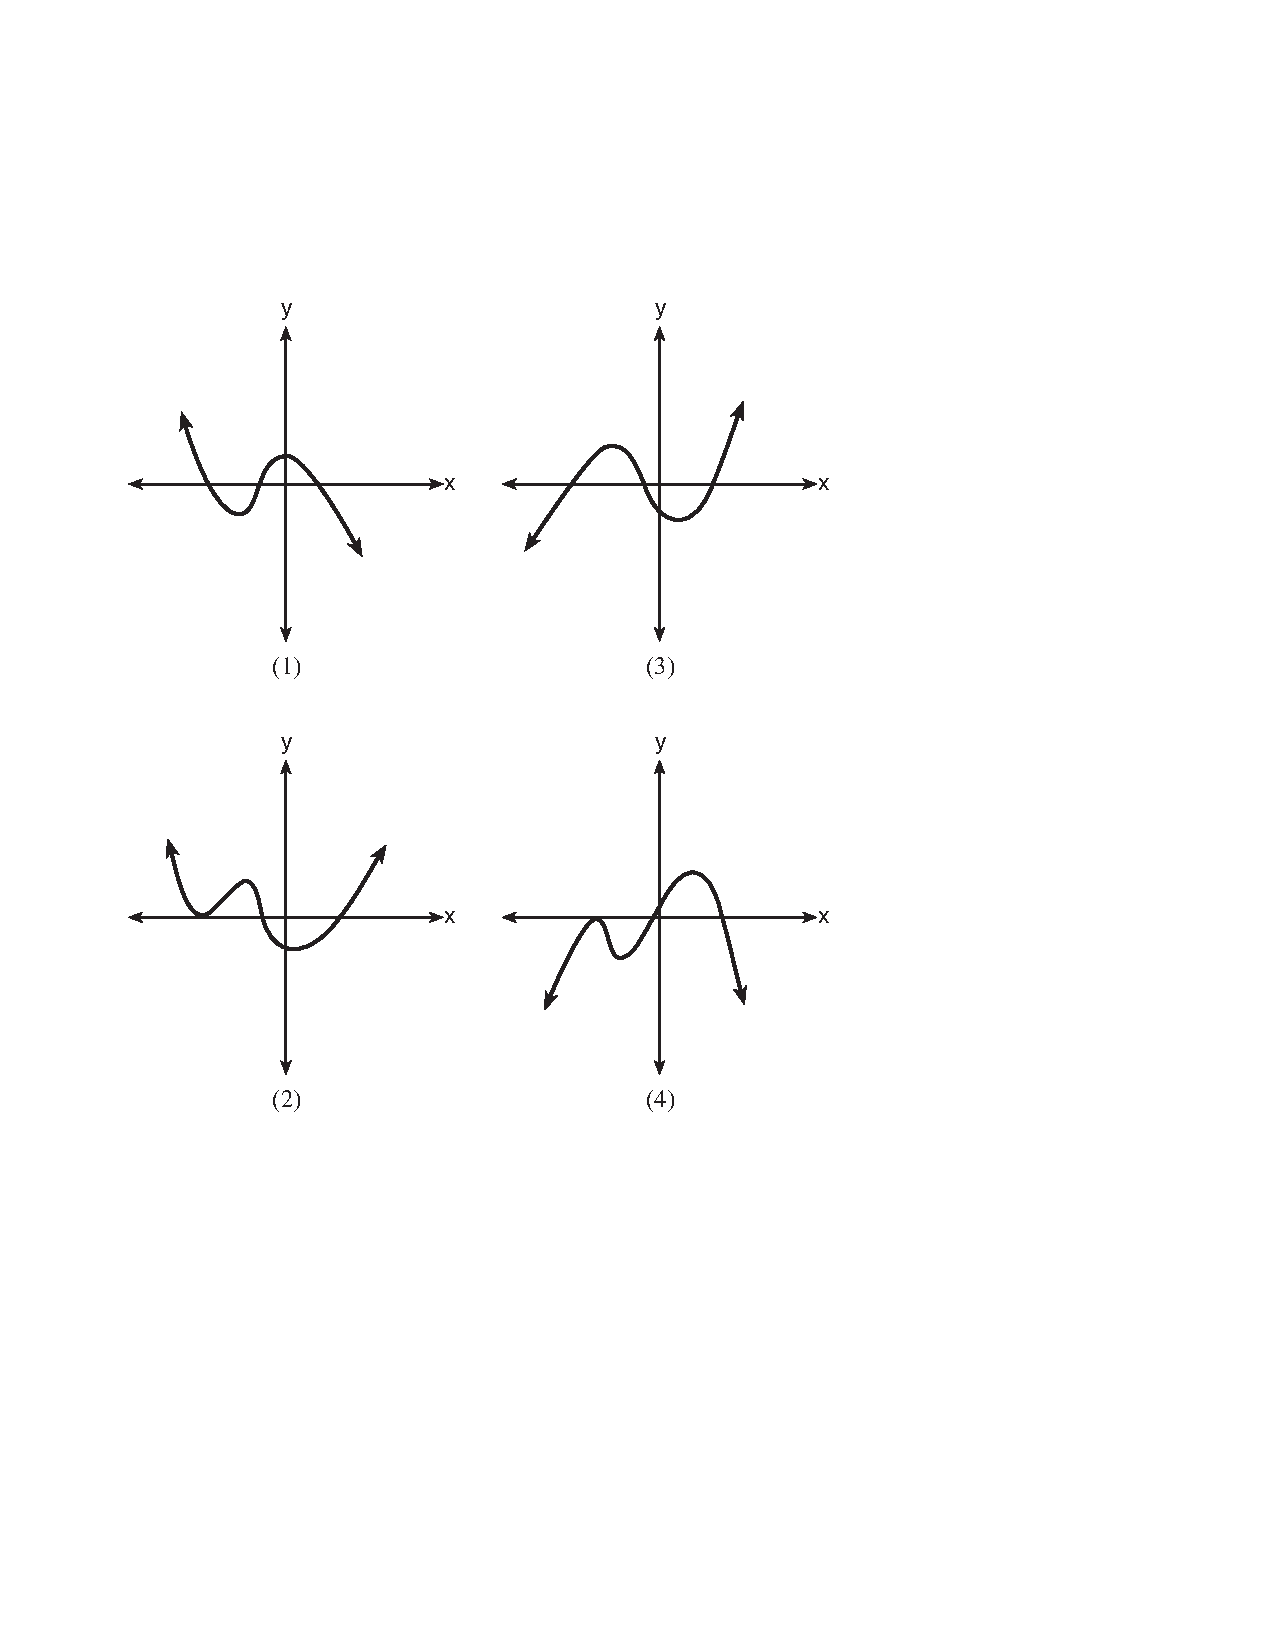
\includegraphics[width=0.75\textwidth]{cubic-graphs.pdf}
\end{figure} %Alg2 Regents Jun2016

\newpage
\item The graph of the function $p(x)$ is sketched below.
\begin{center}
    \begin{tikzpicture}[scale=2.54/4]
    \draw[thick,<->] (-4.5,0) -- (5.5,0) node[anchor=north west] {\textbf{x}};
    \draw[thick,<->] (0,-6.5) -- (0,3.5) node[anchor=south east] {\textbf{p(x)}};
    \foreach \x in {-1, 1} \draw (\x cm,5pt) -- (\x cm,-5pt) node[anchor=north] {$\x$};
    \foreach \x in {-4,-3,-2, 2, 3, 4} \draw (\x cm,5pt) -- (\x cm,-5pt) node[anchor=north] {};
    %\foreach \y in {5} \draw (1pt,\y cm) -- (-1pt,\y cm) node[anchor=east] {50}; %{$\y$};
    \tkzInit[xmin=-5,xmax=5,ymin=-6,ymax=3,ystep=1]   
    \tkzFct[color=black,very thick,<->,domain = -3.2:4] {-0.2*(x*x-9)*(x-2)};
    \end{tikzpicture}
\end{center}
Which equation could represent $p(x)$?
\begin{enumerate}
    \item $p(x)=(x^2+ 9)(x-2)$
    \item $p(x)=x^3 -2x^2+ 9x+18$
    \item $p(x)=(x^2- 9)(x-2)$
    \item $p(x)=x^3 +2x^2- 9x-18$
\end{enumerate} %Alg2 Regents Jun2017 multiple choice

\item When $g(x)$ is divided by $x-1$, the remainder is 0. Given $g(x)= x^4+3x^3-6x^2-6x+8$, which conclusion about $g(x)$ is true?
\begin{enumerate}
    \item $g(1)=0$
    \item $g(-1)=0$
    \item $x+1$ is a factor of $g(x)$.
    \item No conclusion can be made regarding $g(x)$.
\end{enumerate} %Alg2 Regents Jan2017 multiple choice

\item The expression $\displaystyle \left( \frac{m^2}{m^\frac{1}{3}}\right)^{\frac{1}{2}}$ is equivalent to 
\begin{enumerate}
    \item $\sqrt[6]{m^5}$
    \item $\displaystyle \frac{1}{\sqrt[6]{m^5}}$
    \item $-m \sqrt[5]{m}$
    \item $\displaystyle -\frac{1}{m \sqrt[5]{m}}$
\end{enumerate} %Alg2 Regents Jan2017 multiple choice

\newpage
\item Determine if $x-4$ is a factor of $2x^3-4x^2-7x-10$. Explain your answer. %Jun2016 Regents FR


\end{enumerate}
\end{document}